% Copyright 2004 by Till Tantau <tantau@users.sourceforge.net>.
%
% In principle, this file can be redistributed and/or modified under
% the terms of the GNU Public License, version 2.
%
% However, this file is supposed to be a template to be modified
% for your own needs. For this reason, if you use this file as a
% template and not specifically distribute it as part of a another
% package/program, I grant the extra permission to freely copy and
% modify this file as you see fit and even to delete this copyright
% notice. 

\documentclass[aspectratio=169]{beamer}
\hypersetup{pdfpagemode=FullScreen} % Start in fullscreen mode in adobe acrobat

\usepackage[utf8]{inputenx}
\usepackage[super]{nth}
\usepackage{tikz}
\usetikzlibrary{shapes, arrows, positioning, arrows.meta}
\usepackage{packages/graphiso}   % https://github.com/rvf0068/graphiso.sty, also incluse tkz-graph
\usepackage{booktabs} % Much better 'book style' table spacing
\usepackage{graphicx}
\usepackage{pdfpages}
\usepackage{adjustbox}
\usepackage{forest}
\usepackage{xcolor}
\usepackage[normalem]{ulem}
\usepackage{multirow}
\usepackage{bbding}


% There are many different themes available for Beamer. A comprehensive
% list with examples is given here:
% http://deic.uab.es/~iblanes/beamer_gallery/index_by_theme.html
% You can uncomment the themes below if you would like to use a different
% one:
%\usetheme{AnnArbor}
%\usetheme{Antibes}
%\usetheme{Bergen}
%\usetheme{Berkeley}
%\usetheme{Berlin}
%\usetheme{Boadilla}
%\usetheme{boxes}
\usetheme{CambridgeUS}
%\usetheme{Copenhagen}
%\usetheme{Darmstadt}
% \usetheme{default}
%\usetheme{Frankfurt}
%\usetheme{Goettingen}
%\usetheme{Hannover}
% \usetheme{Ilmenau}
%\usetheme{JuanLesPins}
%\usetheme{Luebeck}
% \usetheme{Madrid}
%\usetheme{Malmoe}
%\usetheme{Marburg}
% \usetheme{Montpellier}
%\usetheme{PaloAlto}
%\usetheme{Pittsburgh}
%\usetheme{Rochester}
% \usetheme{Singapore}
%\usetheme{Szeged}
% \usetheme{Warsaw}

\title{Graph Isomorphisms \& Automorphisms}

% A subtitle is optional and this may be deleted
\subtitle{University of Twente \& Nedap University\\Nedap University 2016--2018 graduation}

% Tussen voorletters kan een smallere spatie, te weten: \,
\author[]{A.\,G.~van~Herwijnen \and C.\,A.\,M.\,A.~Reuvers \and F.\,T.\,F.~Meijer~Cluwen \and\\M.\,H.\,B.~Banierink \and M.\,M.~Slot \and E.~Huizinga}

\date[NU2 Graduation, 23-04-2018]{23-04-2018}

\subject{Discrete Structures and Efficient Algorithms}

\newcommand{\dy}{5cm}
\newcommand{\darkarrow}{{Latex[length=4mm, width=3mm]}}

\setbeamertemplate{enumerate items}[circle]
\setbeamertemplate{itemize items}[circle]

% Change colours
\definecolor{orange}{RGB}{255, 135, 0}

\setbeamercolor{frametitle}{fg=orange}
\setbeamercolor{title}{fg=orange}
\setbeamercolor{palette primary}{fg=orange!80!, bg=gray!30!white} 
\setbeamercolor{palette secondary}{fg=orange!80!, bg=gray!20!white}
\setbeamercolor{palette tertiary}{fg=white!80!, bg=orange}

\setbeamercolor{item projected}{fg=white, bg=orange}
\setbeamercolor{subitem projected}{fg=white, bg=orange}
\setbeamercolor{subsubitem projected}{fg=white, bg=orange}
\setbeamercolor{itemize item}{fg=orange}
\setbeamercolor{itemize subitem}{fg=orange}
\setbeamercolor{itemize subsubitem}{fg=orange}
\setbeamercolor{alerted text}{fg=orange}

% Change margin
\setbeamersize{text margin left=20pt,text margin right=15pt}

% Let's get started
\begin{document}
\setbeamertemplate{caption}{\raggedright\insertcaption\par}
\beamertemplatenavigationsymbolsempty

\begin{frame}
  \titlepage
\end{frame}

% \begin{frame}{Outline}
%   \tableofcontents
% %   You might wish to add the option [pausesections]
% \end{frame}

% \section{First Main Section}

\subsection{First Subsection}

\begin{frame}{First Slide Title}{Optional Subtitle}
  \begin{itemize}
  \item {
    My first point.
  }
  \item {
    My second point.
  }
  \end{itemize}
\end{frame}

\subsection{Second Subsection}

% You can reveal the parts of a slide one at a time
% with the \pause command:
\begin{frame}{Second Slide Title}
  \begin{itemize}
  \item {
    First item.
    \pause % The slide will pause after showing the first item
  }
  \item {   
    Second item.
  }
  % You can also specify when the content should appear
  % by using <n->:
  \item<3-> {
    Third item.
  }
  \item<4-> {
    Fourth item.
  }
  % or you can use the \uncover command to reveal general
  % content (not just \items):
  \item<5-> {
    Fifth item. \uncover<6->{Extra text in the fifth item.}
  }
  \end{itemize}
\end{frame}

\section{Second Main Section}

\subsection{Another Subsection}

\begin{frame}{Blocks}
\begin{block}{Block Title}
You can also highlight sections of your presentation in a block, with it's own title
\end{block}
\begin{theorem}
There are separate environments for theorems, examples, definitions and proofs.
\end{theorem}
\begin{example}
Here is an example of an example block.
\end{example}
\end{frame} % Uncomment this line to see the demo slides from beamer
\section{Introduction}
\begin{frame}{Graphs for dummies}
    \begin{itemize}
        \uncover<1->{\item Vertex}
        \uncover<3->{\item Edge}
        \uncover<4->{\item Graph}
        \begin{itemize}
            \uncover<5->{\item Undirected vs.\ directed}
            \uncover<6->{\item Simple vs.\ multi-edge}
        \end{itemize}
    \end{itemize}
    
    \centering
    \begin{tikzpicture}
        \uncover<1->{\Vertex{1}}
        \uncover<2->{\EA[unit=3](1){2}}
        \uncover<3-4,7>{\Edge(1)(2)}
        \uncover<5>{\Edge[style={-\darkarrow}](1)(2)}
        \uncover<6>{\Edge[style={bend right=30}](1)(2)}
        \uncover<6>{\Edge[style={bend right=-30}](1)(2)}
    \end{tikzpicture}
    
    \uncover<7->{We only consider simple, undirected graphs}
\end{frame}

\begin{frame}{What is graph isomorphism?}
    \begin{center}
    \begin{tikzpicture}
        {\renewcommand{\VertexLightFillColor}{orange}\Vertex[x=0,y=-2.8]{1}}
        {\renewcommand{\VertexLightFillColor}{red}\Vertex[x=-3,y=-1]{2}}
        {\renewcommand{\VertexLightFillColor}{yellow}\Vertex[x=0,y=-1]{3}}
        {\renewcommand{\VertexLightFillColor}{green}\Vertex[x=3,y=-1]{4}}
        {\renewcommand{\VertexLightFillColor}{blue}\Vertex[x=-4,y=1, style=blue]{5}}
        {\renewcommand{\VertexLightFillColor}{purple}\Vertex[x=-2,y=1]{6}}
        {\renewcommand{\VertexLightFillColor}{pink}\Vertex[x=-1,y=1]{7}}
        {\renewcommand{\VertexLightFillColor}{magenta}\Vertex[x=1,y=1]{8}}
        {\renewcommand{\VertexLightFillColor}{lime}\Vertex[x=2,y=1]{9}}
        {\renewcommand{\VertexLightFillColor}{cyan}\Vertex[x=4,y=1]{10}}        
        
        \Edge(2)(1)
        \Edge(3)(1)
        \Edge(4)(1)
        \Edge(2)(5)
        \Edge(2)(6)
        \Edge(3)(7)
        \Edge(3)(8)
        \Edge(4)(9)
        \Edge(4)(10)
        \Edge(8)(9)

        % Now some curved edges
        \Edge[style = {bend left=60}](5)(7)
        \Edge[style = {bend left=60}](5)(9)
        \Edge[style = {bend left=60}](6)(8)
        \Edge[style = {bend left=60}](6)(10)
        \Edge[style = {bend left=60}](6)(8)
        \Edge[style = {bend left=60}](6)(10)
        \Edge[style = {bend left=60}](7)(10)
    \end{tikzpicture}
  \end{center}
\end{frame}
\begin{frame}
    \transduration{0.25}
    \begin{center}
    \begin{tikzpicture}[stop jumping]
      % Vertex 1 appears at slide 1
      {\renewcommand{\VertexLightFillColor}{orange}\VertexM[xa=0,ya=-2.8,xb=3*cos(234),yb=3*sin(234),starts=1,stops=10]{1}}
      {\renewcommand{\VertexLightFillColor}{red}\VertexM[xa=-3,ya=-1,xb=3*cos(162),yb=3*sin(162),starts=1,stops=10]{2}}
      {\renewcommand{\VertexLightFillColor}{yellow}\VertexM[xa=0,ya=-1,xb=1.5*cos(234),yb=1.5*sin(234),starts=1,stops=10]{3}}
      {\renewcommand{\VertexLightFillColor}{green}\VertexM[xa=3,ya=-1,xb=3*cos(306),yb=3*sin(306),starts=1,stops=10]{4}}
      % Edges from 1 to 2,3,4. Since no bending is needed, they are simple \Edge commands
      \Edge(2)(1)
      \Edge(3)(1)
      \Edge(4)(1)

      % Vertices 5,6,7,8,9,10 appear at slide 3, also some simple edges
      {\renewcommand{\VertexLightFillColor}{blue}\VertexM[xa=-4,ya=1,xb=3*cos(90),yb=3*sin(90),starts=1,stops=10]{5}}
      {\renewcommand{\VertexLightFillColor}{purple}\VertexM[xa=-2,ya=1,xb=1.5*cos(162),yb=1.5*sin(162),starts=1,stops=10]{6}}
      \Edge(2)(5)
      \Edge(2)(6)
      {\renewcommand{\VertexLightFillColor}{pink}\VertexM[xa=-1,ya=1,xb=1.5*cos(90),yb=1.5*sin(90),starts=1,stops=10]{7}}
      {\renewcommand{\VertexLightFillColor}{magenta}\VertexM[xa=1,ya=1,xb=1.5*cos(18),yb=1.5*sin(18),starts=1,stops=10]{8}}
      \Edge(3)(7)
      \Edge(3)(8)
      {\renewcommand{\VertexLightFillColor}{lime}\VertexM[xa=2,ya=1,xb=3*cos(18),yb=3*sin(18),starts=1,stops=10]{9}}
      {\renewcommand{\VertexLightFillColor}{cyan}\VertexM[xa=4,ya=1,xb=1.5*cos(306),yb=1.5*sin(306),starts=1,stops=10]{10}}
      \Edge(4)(9)
      \Edge(4)(10)

      % Now some curved edges, appearing in slides 6,7,8. We use the
      % default values: bends=left, bendsfrom=60
      \EdgeM[starts=1,stops=10]{5}{7}
      \EdgeM[starts=1,stops=10]{5}{9}

      \EdgeM[starts=1,stops=10]{6}{8}
      \EdgeM[starts=1,stops=10]{6}{10}

      \EdgeM[starts=1,stops=10]{6}{8}
      \EdgeM[starts=1,stops=10]{6}{10}

      \EdgeM[starts=1,stops=10]{7}{10}

      % The last edge to appear is a simple one
      \Edge(8)(9)
    \end{tikzpicture}
    \pause
  \end{center}
\end{frame}
\begin{frame}
    \begin{center}
    \pgfmathsetmacro{\cosi}{cos(234)}
    \pgfmathsetmacro{\sini}{sin(234)}
    \pgfmathsetmacro{\cosii}{cos(162)}
    \pgfmathsetmacro{\sinii}{sin(162)}
    \pgfmathsetmacro{\cosiii}{cos(90)}
    \pgfmathsetmacro{\siniii}{sin(90)}
    \pgfmathsetmacro{\cosiiii}{cos(18)}
    \pgfmathsetmacro{\siniiii}{sin(18)}
    \pgfmathsetmacro{\cosiiiii}{cos(306)}
    \pgfmathsetmacro{\siniiiii}{sin(306)}
    \begin{tikzpicture}
      {\renewcommand{\VertexLightFillColor}{orange}\Vertex[x=3*\cosi ,y=3*\sini]{1}}
      {\renewcommand{\VertexLightFillColor}{red}\Vertex[x=3*\cosii,y=3*\sinii]{2}}
      {\renewcommand{\VertexLightFillColor}{yellow}\Vertex[x=1.5*\cosi,y=1.5*\sini]{3}}
      {\renewcommand{\VertexLightFillColor}{green}\Vertex[x=3*\cosiiiii,y=3*\siniiiii]{4}}
    %   % Edges from 1 to 2,3,4. Since no bending is needed, they are simple \Edge commands
      \Edge(2)(1)
      \Edge(3)(1)
      \Edge(4)(1)

    %   % Vertices 5,6,7,8,9,10 appear at slide 3, also some simple edges
      {\renewcommand{\VertexLightFillColor}{blue}\Vertex[x=3*\cosiii,y=3*\siniii]{5}}
      {\renewcommand{\VertexLightFillColor}{purple}\Vertex[x=1.5*\cosii,y=1.5*\sinii]{6}}
      \Edge(2)(5)
      \Edge(2)(6)
      {\renewcommand{\VertexLightFillColor}{pink}\Vertex[x=1.5*\cosiii,y=1.5*\siniii]{7}}
      {\renewcommand{\VertexLightFillColor}{magenta}\Vertex[x=1.5*\cosiiii,y=1.5*\siniiii]{8}}
      \Edge(3)(7)
      \Edge(3)(8)
      {\renewcommand{\VertexLightFillColor}{lime}\Vertex[x=3*\cosiiii,y=3*\siniiii]{9}}
      {\renewcommand{\VertexLightFillColor}{cyan}\Vertex[x=1.5*\cosiiiii,y=1.5*\siniiiii]{10}}
      \Edge(4)(9)
      \Edge(4)(10)

      \Edge(5)(7)
      \Edge(5)(9)
      \Edge(6)(8)
      \Edge(6)(10)
      \Edge(7)(10)
      \Edge(8)(9)
    \end{tikzpicture}
  \end{center}
\end{frame}

\begin{frame}{Introduction}
\begin{enumerate}[<+->]
  \item {
    Graph Isomorphism problem
    \begin{itemize}
        \item\uncover Why do we need it?
        \item\uncover Solvable in polynomial time?
    \end{itemize}
  }
  \item Number of automorphisms problem
\end{enumerate}
\end{frame}


\section{Solving the problem}

%\subsection*{Processing pipeline}
\subsection*{}
\begin{frame}<1-2>[label=processing-overview]{Processing pipeline overview}
    \tikzstyle{cloud} = [circle, draw, text width=5em, text centered]
    \tikzstyle{line} = [draw, -\darkarrow, thick]
    \tikzstyle{block} = [draw, rectangle, fill = red!20, text width = 4cm, text centered, minimum height = 3cm]
    
    \adjustbox{max width = \textwidth}{
        \begin{tikzpicture}[node distance = 1.5cm]
            \node<-2> [cloud, fill = blue!20] (graphs) {Set of graphs};
            \node<3-> [opacity = .2, cloud, fill = blue!20] (graphs) {Set of graphs};
            
            \node<1> [block, right = of graphs] (proiso) {Process graphs pairwise into isomorphic groups};
            \node<2> [block, right = of graphs, line width = 0.5mm] (proiso) {Process graphs pairwise into isomorphic groups};
            \node<3-> [opacity = .2, block, right = of graphs] (proiso) {Process graphs pairwise into isomorphic groups};
            
            \node<1> [block, right = of proiso] (proauto) {Calculate number of authomorphisms of one graph per isomorphic group};
            \node<3> [block, right = of proiso, line width = 0.5mm] (proauto) {Calculate number of authomorphisms of one graph per isomorphic group};
            \node<2, 4-> [block, opacity=0.2, right = of proiso] (proauto) {Calculate number of authomorphisms of one graph per isomorphic group};
            
            \node<1> [cloud, fill = green!20, right = of proauto] (results) {Results};
            \node<4> [cloud, fill = green!20, right = of proauto, line width = 0.5mm] (results) {Results};
            \node<2-3> [cloud, opacity = .2, fill = green!20, right = of proauto] (results) {Results};
            
            \path<-2> [line] (graphs) -- (proiso);
            \path<3-> [opacity = .2, line] (graphs) -- (proiso);
            
            \path<1, 3> [line] (proiso) -- (proauto);
            \path<2, 4> [opacity = .2, line] (proiso) -- (proauto);
            
            \path<1, 4> [line] (proauto) -- (results);
            \path<2-3> [opacity = .2, line] (proauto) -- (results);
        \end{tikzpicture}
    }
\end{frame}


\subsection*{}
\begin{frame}<1-2>[label=flow]{GI processing pipeline}
    \tikzstyle{cloud} = [circle, draw, text width=5em, text centered, minimum height=4em, node distance=3cm, inner sep=0pt]
    \tikzstyle{test} = [diamond, draw, aspect=2, fill=orange!20, text width = 5em, minimum width = 4cm, minimum height = 2cm, inner sep=1pt, align=center]
    \tikzstyle{line} = [draw, thick]
    \tikzstyle{line-with-arrow} = [line, -\darkarrow]
    \tikzstyle{block} = [draw, rectangle ,fill=blue!20, node distance=3cm, minimum height=2em, text width=6em, text centered, minimum height=4em]
    
    \centering

    \adjustbox{max height = \dimexpr\textheight-2cm, max width=\textwidth}{
        \begin{tikzpicture}[auto]
            
            \only<1->{
                \node [cloud, fill=yellow!20] (graphs) at (canvas cs:x=0cm,y=0cm) {Graphs $G$ and $H$};
                \node [cloud, fill=red!20] (isnotiso) at (canvas cs:x=6cm,y=0cm) {Assign $G$~and~$H$ \textbf{in~different} isomorphic groups};
                \node [cloud, fill=green!20] (isiso) at (canvas cs:x=12cm, y=0cm) {Assign $G$~and~$H$ \textbf{in~the~same} isomorphic group};
            }
            
            \only<1, 4->{
                \node [test] (preproc) at (canvas cs:x=0cm, y=-4cm) {Preprocess graphs};
            }
            
            \only<1, 6->{
                \node [test] (areconnected) at (canvas cs:x=0cm, y=-8cm) {Determine connectivity};
            }
            
            \only<1, 7->{
                \node [test] (istree1) at (canvas cs:x=12cm, y=-8cm) {Determine if trees};
            }
            
            \only<1, 9->{
                \node [test] (moddec) at (canvas cs:x=20cm, y=-8cm) {Modular decomposition};
            }
            
            \only<1, 10->{
                \node [test] (istree2) at (canvas cs:x=20cm, y=-4cm) {Determine if trees};
            }
            
            \only<1, 12->{
                \node [test] (treeproc) at (canvas cs:x=12cm,y=-4cm) {Process trees};
            }
            
            \only<1, 14->{
                \node [test] (colorref) at (canvas cs:x=20cm, y=0cm) {Use color refinement \& branching};
            }
            
            \only<2-3>{
                \node [test, opacity=0.2] (areconnected) at (canvas cs:x=0cm, y=-8cm) {Determine connectivity};
            }
            
            \only<2-5>{
                \node [test, opacity=0.2] (istree1) at (canvas cs:x=12cm, y=-8cm) {Determine if trees};
            }
            
            \only<2-6>{
                \node [test, opacity=0.2] (moddec) at (canvas cs:x=20cm, y=-8cm) {Modular decomposition};
            }
            
            \only<2-8>{
                \node [test, opacity=0.2] (istree2) at (canvas cs:x=20cm, y=-4cm) {Determine if trees};
            }
            
            \only<2-9>{
                \node [test, opacity=0.2] (treeproc) at (canvas cs:x=12cm,y=-4cm) {Process trees};
            }
            
            \only<2-11>{
                \node [test, opacity=0.2] (colorref) at (canvas cs:x=20cm, y=0cm) {Use color refinement \& branching};
            }

            \only<2-3>{
                \node [test, line width = 1mm] (preproc) at (canvas cs:x=0cm, y=-4cm) {Preprocess graphs};
            }
            
            \only<4-5>{
                \node[test, line width = 1mm] (areconnected) at (canvas cs:x=0cm, y=-8cm) {Determine connectivity};
            }
            
            \only<6>{
                \node[test, line width = 1mm] (istree1) at (canvas cs:x=12cm, y=-8cm) {Determine if trees};
            }
            
            \only<7-8>{
                \node [test, line width = 1mm] (moddec) at (canvas cs:x=20cm, y=-8cm) {Modular decomposition};
            }
            
            \only<9>{
                \node[test, line width = 1mm] (istree2) at (canvas cs:x=20cm, y=-4cm) {Determine if trees};
            }
            
            \only<10-11>{
                \node [test, line width = 1mm] (treeproc) at (canvas cs:x=12cm,y=-4cm) {Process trees};
            }
            
            \only<12-13>{
                \node [test, line width = 1mm] (colorref) at (canvas cs:x=20cm, y=0cm) {Use color refinement \& branching};
            }
            
            \only<1->{
                \path [line-with-arrow] (graphs) -- (preproc);
                \path[line-with-arrow] (preproc) -- node [] {not isomorphic} +(6cm, 0);
                \path [line-with-arrow] +(6cm, -4cm) -- (isnotiso);
                \path[line-with-arrow] (preproc) -- node [near start] {possibly isomorphic} (areconnected);
            }
            
            \only<1, 4->{
                \path [line-with-arrow] (areconnected) -| ++(-3, 2) |- node [near start, rotate=90, yshift=1em, xshift=2em] {same \# components} (preproc);
                \path [line-with-arrow] (areconnected) |- ++(0, -2) -| node [near start] {both connected} (istree1);
                \path [line-with-arrow] (areconnected) -- node [align = left] {different\\\# components} +(6cm, 0cm);
                \path [line] +(6cm, -8cm) -- +(6cm, -4cm);
            }
            
            \only<1, 6->{
                \path[line-with-arrow] (istree1) -- node [] {both not trees} (moddec);
                \path[line-with-arrow] (istree1) -- node [near start] {both are trees} (treeproc);
                \path[line-with-arrow] (istree1) -- node [] {only one tree} +(-6cm, 0);
            }
            
            \only<1, 7->{
                \path[line-with-arrow] (moddec) -- node [near start] {similar decompositions}(istree2);
                \path[line-with-arrow] (moddec) -| node [near start, xshift=0em, align = left] {different\\decom-\\positions} +(4cm, 4cm);
                \path [line-with-arrow] +(24cm, -4cm) |- +(20cm, 3cm);
                \path [line-with-arrow] +(20cm, 3cm) -| (isnotiso);
            }
            
            \only<1, 9->{
                \path[line-with-arrow] (istree2) -- node [align = left] {only one\\tree} +(4cm, 0cm);
                \path[line-with-arrow] (istree2) -- node [] {both are trees} (treeproc);
                \path[line-with-arrow] (istree2) -- node [near start] {both not trees} (colorref);
            }
            
            \only<1, 10->{
                \path[line-with-arrow] (treeproc) -- node [near start] {isomorphic} (isiso);
                \path[line-with-arrow] (treeproc) -- node [] {not isomorphic} +(-6cm, 0); +(4cm, 4cm);
            }
            
            \only<1, 12->{
                \path [line-with-arrow] (colorref) -- node [] {isomorphic} (isiso);
                \path [line-with-arrow] (colorref) -- node [near start] {not isomorphic} +(0, 3cm);
            }

            \only<2-3>{
                \path [line-with-arrow, opacity=.2] (areconnected) -| ++(-3, 2) |- node [near start, rotate=90, yshift=1em, xshift=2em] {same \# components} (preproc);
                \path [line-with-arrow, opacity=.2] (areconnected) |- ++(0, -2) -| node [near start] {both connected} (istree1);
                \path [line-with-arrow, opacity=.2] (areconnected) -- node [align = left] {different\\\# components} +(6cm, 0cm);
                \path [line, opacity=.2] +(6cm, -8cm) -- +(6cm, -4cm);
            }
            
            \only<2-5>{
                \path[line-with-arrow, opacity=.2] (istree1) -- node [] {both not trees} (moddec);
                \path[line-with-arrow, opacity=.2] (istree1) -- node [near start] {both are trees} (treeproc);
                \path[line-with-arrow, opacity=.2] (istree1) -- node [] {only one tree} +(-6cm, 0);
            }
            
            \only<2-6>{
                \path[line-with-arrow, opacity=.2] (moddec) -- node [near start] {similar decompositions}(istree2);
                \path[line-with-arrow, opacity=.2] (moddec) -| node [near start, xshift=0em, align = left] {different\\decom-\\positions} +(4cm, 4cm);
                \path [line-with-arrow, opacity=.2] +(24cm, -4cm) |- +(20cm, 3cm);
                \path [line-with-arrow, opacity=.2] +(20cm, 3cm) -| (isnotiso);
            }
            
            \only<2-8>{
                \path[line-with-arrow, opacity=.2] (istree2) -- node [align = left] {only one\\tree} +(4cm, 0cm);
                \path[line-with-arrow, opacity=.2] (istree2) -- node [] {both are trees} (treeproc);
                \path[line-with-arrow, opacity=.2] (istree2) -- node [near start] {both not trees} (colorref);
            }
            
            \only<2-9>{
                \path[line-with-arrow, opacity=.2] (treeproc) -- node [near start] {isomorphic} (isiso);
                \path[line-with-arrow, opacity=.2] (treeproc) -- node [] {not isomorphic} +(-6cm, 0); +(4cm, 4cm);
            }
            
            \only<2-11>{
                \path [line-with-arrow, opacity=.2] (colorref) -- node [] {isomorphic} (isiso);
                \path [line-with-arrow, opacity=.2] (colorref) -- node [near start] {not isomorphic} +(0, 3cm);
            }
            
        \end{tikzpicture}
    }
\end{frame}


\subsection{Preprocessing}

\begin{frame}{Preprocessing}
    \tikzstyle{block} = [rectangle, draw, fill=orange!40, 
    text width=5em, text centered, minimum height=4em]
    \tikzstyle{line} = [draw, -\darkarrow]
    \newcommand*\activelinewidth{0.5mm}
    \begin{center}
    \begin{tikzpicture}[node distance = 3cm]
        \node<1>[block, line width = \activelinewidth] (start) {Size};
        \node<2->[block, line width = 0.15mm] (start) {Size};
        \node<2>[block, line width = \activelinewidth ,right of=start](order) {Order};
        \node<1>[block, line width = 0.15mm ,right of=start, opacity = 0.2](order) {Order};
        \node<3->[block, line width = 0.15mm ,right of=start](order) {Order};
        \node<3>[block, line width = \activelinewidth,right of=order](degree) {Degree distribution};
        \node<1-2>[block, line width = 0.15mm,right of=order, opacity = 0.2](degree) {Degree distribution};
        \node<4->[block, line width = 0.15mm,right of=order](degree) {Degree distribution};
        \node<4>[block, line width = \activelinewidth,right of=degree] (compl) {Complement};
        \node<1-3>[block, line width = 0.15mm,right of=degree, opacity = 0.2] (compl) {Complement};
        % % Draw edges
        \path<1>[line,opacity = 0.2] (start) -- (order);
        \path<1-2>[line,opacity = 0.2] (order) -- (degree);
        \path<1-3>[line,opacity = 0.2] (degree) -- (compl);
        \path<2->[line] (start) -- (order);
        \path<3->[line] (order) -- (degree);
        \path<4->[line] (degree) -- (compl);
    \end{tikzpicture}
    \end{center}
    \only<1-3>{
        \begin{figure}
        \begin{tikzpicture}
            \Vertices{circle}{A,B,C}
            \Edges(A,B,C)
        \end{tikzpicture}
        \caption{\only<1>{Size = 2}
        \only<2>{Order = 3}
        \only<3>{deg = 1: (A,C), deg = 2: (B)}}
        \end{figure}
    }
    \only<4>{
    \begin{figure}
    \begin{minipage}{0.35\textwidth}
        \centering
        \begin{tikzpicture}
            \Vertices{square}{A,B,C,D}
            \Edges(A,C,B,D,A)
        \end{tikzpicture}
        \caption{Original graph}
    \end{minipage}
    \begin{minipage}{0.35\textwidth}
        \centering
        \begin{tikzpicture}
            \Vertices{square}{A,B,C,D}
            \Edge(C)(D)
            \Edge(A)(B)
        \end{tikzpicture}
    \caption{Complement}
    \end{minipage}
    \end{figure}
    }
\end{frame}

\subsection{}
\againframe<3-4>{flow}

\subsection{Connectivity}

\begin{frame}{Connectivity}
    \begin{enumerate}
        \item Keep track of visited vertices
        \item Select any unvisited vertex
        \item Start Breadth First Search from this vertex
        \uncover<4-7>{\item If there are still unvisited vertices, there is another component}
    \end{enumerate}
    
    \centering
    \tikzstyle{vertex}=[circle, draw, minimum size=15pt]
    \begin{tikzpicture}[auto]
        \node<1>[vertex](0) at (0,0){0};
        \node<2->[vertex, fill=orange](0) at (0,0){0};
        \node<-2>[vertex](1) at (0,2){1}; 
        \node<3->[vertex, fill=orange](1) at (0,2){1};
        \node<-3>[vertex](2) at (2,2){2};
        \node<4->[vertex, fill=orange](2) at (2,2){2};
        \node<-2>[vertex](3) at (1,1){3};
        \node<3->[vertex, fill=orange](3) at (1,1){3};
        
        \node<-4>[vertex](4) at (3,0){4}; 
        \node<-5>[vertex](5) at (4,1){5};
        \node<-6>[vertex](6) at (5,2){6};
        \node<5->[vertex, fill = lime](4) at (3,0){4}; 
        \node<6->[vertex, fill = lime](5) at (4,1){5};
        \node<7->[vertex, fill = lime](6) at (5,2){6};
        
        \Edge (0)(1);
        \Edge (0)(3);
        \Edge (3)(1);
        \Edge (3)(2);
        \Edge (4)(5);
        \Edge (5)(6);
    \end{tikzpicture}
        
    \centering
    \uncover<2->{%
        Visited = [\only<2->{0}\only<3->{, 1, 3}\only<4->{, 2}\only<5->{, 4}\only<6->{, 5}\only<7->{, 6}]
        
        Number of components = \only<1-4>{1}\only<5->{2}
    }
\end{frame}
\subsection{}
\againframe<5-7>{flow}

\subsection{Modular decomposition}
\begin{frame}{Modular decomposition}
    \begin{itemize}
        \item Simplify graph by grouping similar vertices, i.\,e.\ modules, into one vertex
        \uncover<2->{\item Vertices are grouped by neighbourhood}
    \end{itemize}
    \uncover<3->{
        \begin{center}
            \begin{tikzpicture}
                \Vertex[x=-6, y=0]{1}
                \Vertex[x=-3, y=0]{3}
                \Vertex[x=0, y=0]{5}
                \Vertex[x=3, y=0]{11}
                
                \uncover<3-8>{
                    \Vertex[x=-7.5, y=1]{0}
                    \Vertex[x=-7.5, y=-1]{10}
                    \Edge(0)(1)
                    \Edge(10)(1)
                }
                
                \uncover<3-9>{
                    \Vertex[x=-4.5, y=1]{2}
                    \Vertex[x=-4.5, y=-1]{9}
                    \Edge(2)(1)
                    \Edge(9)(1)
                    \Edge(2)(9)
                    \Edge(2)(3)
                    \Edge(9)(3)
                }
                
                \uncover<3-10>{
                    \Vertex[x=-1.5, y=1]{4}
                    \Vertex[x=-1.5, y=-1]{8}
                    \Edge(4)(3)
                    \Edge(3)(8)
                    \Edge(4)(5)
                    \Edge(8)(5)
                }
                
                \uncover<3-11>{
                    \Vertex[x=1.5, y=1]{6}
                    \Vertex[x=1.5, y=-1]{7}
                    \Edge(6)(5)
                    \Edge(7)(5)
                    \Edge(6)(7)
                    \Edge(6)(11)
                    \Edge(7)(11)
                }
                
                \uncover<3-12>{
                    \Vertex[x=4.5, y=1]{12}
                    \Vertex[x=4.5, y=-1]{14}
                    \Vertex[x=6, y=0]{13}
                    \Edge(11)(12)
                    \Edge(11)(14)
                    \Edge(11)(13)
                    \Edge(12)(14)
                    \Edge(12)(13)
                    \Edge(13)(14)
                }
                
                \uncover<4-8>{
                    \draw[green, rounded corners=10pt, line width=2pt] (-8,-2) rectangle (-7,2);
                }
                
                \uncover<5-9>{
                    \draw[red, rounded corners=10pt, line width=2pt] (-5,-2) rectangle (-4,2);
                }
                
                \uncover<6-10>{
                    \draw[green, rounded corners=10pt, line width=2pt] (-2,-2) rectangle (-1,2);
                }
                
                \uncover<7-11>{
                    \draw[red, rounded corners=10pt, line width=2pt] (1,-2) rectangle (2,2);
                }
                
                \uncover<8-12>{
                    \draw[blue, rounded corners=10pt, line width=2pt] (3.75,-2) rectangle (6.5,2);
                }
                
                \newcommand{\oldVertexLineWidth}{\VertexLineWidth}
                \newcommand{\oldVertexLineColor}{\VertexLineColor}
                
                \renewcommand*{\VertexLineWidth}{1.6pt}
                
                \uncover<9->{
                    \renewcommand*{\VertexLineColor}{green}
                    \WE[unit=1.5, Math, L={0||10}](1){MD1+10}
                    \Edge(1)(MD1+10)
                }
                
                \uncover<10->{
                    \renewcommand*{\VertexLineColor}{red}
                    \WE[unit=1.5, L={2--9}](3){MD2+9}
                    \Edge(1)(MD2+9)
                    \Edge(3)(MD2+9)
                }
                
                \uncover<11->{
                    \renewcommand*{\VertexLineColor}{green}
                    \WE[unit=1.5, Math, L={4||8}](5){MD4+8}
                    \Edge(3)(MD4+8)
                    \Edge(5)(MD4+8)
                }
                
                \uncover<12->{
                    \renewcommand*{\VertexLineColor}{red}
                    \WE[unit=1.5, L={6--7}](11){MD6+7}
                    \Edge(5)(MD6+7)
                    \Edge(11)(MD6+7)
                }
                
                \uncover<13->{
                    \renewcommand*{\VertexLineColor}{blue}
                    \EA[unit=2, L={12--13--14}](11){MD12+13+14}
                    \Edge(11)(MD12+13+14)
                }
                
                \renewcommand*{\VertexLineColor}{\oldVertexLineColor}
                \renewcommand*{\VertexLineWidth}{\oldVertexLineWidth}
            \end{tikzpicture}
        \end{center}
    }
    \uncover<14->{\centering \raisebox{-.5ex}{\HandRight} This is a tree, albeit a linear one \raisebox{-.5ex}{\HandLeft}\\[3em]}
\end{frame}
\subsection{}
\againframe<8-10>{flow}

\subsection{Tree isomorphism in $\mathcal{O}(n)$}

\begin{frame}{Tree isomorphism}
    \begin{itemize}
        \item Trees are non-cyclic graphs
        \item Solution for the GI problem in linear time
        \item Good combination with modular decomposition
    \end{itemize}
\end{frame}

\begin{frame}{From graph to rooted tree}
    Algorithm by Bonany \cite{bonamy2010small}, returns the root that splits the tree in half
    \begin{enumerate}
        \item Choose an arbitrary root $r$
        \item Assign each vertex the weight of its induced subtree
        \item Start at $r$ and shift it with the neighbour that has weight \(>\frac{n}{2}\)
    \end{enumerate}
\end{frame}

\begin{frame}{Initial graph}
    \centering
    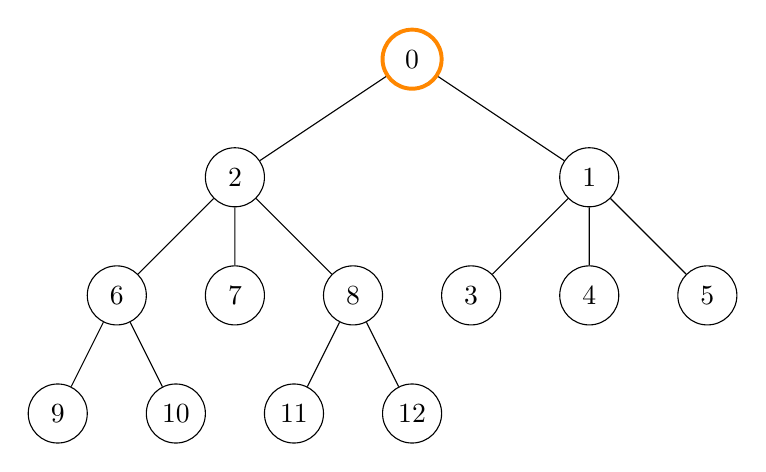
\begin{tikzpicture}[level/.style={sibling distance=15mm},  every node/.style={ minimum size=0.75cm}]
    \node [circle,draw=orange, line width = 0.5mm] (z){0}
        child {node [circle, draw] (y) {2}
            child {node [circle,draw] (a){6}
                child {node [circle,draw] (i) {9}}
                child {node [circle,draw] (j) {10}}
            }
            child {node [circle,draw] (b) {7}}
            child {node [circle,draw] (c) {8}
                child {node [circle,draw] (k) {11}}
                child {node [circle,draw] (l) {12}}
            }
        }
        child {node {} edge from parent[draw=none]}
        child {node {} edge from parent[draw=none]}
        child {node [circle,draw] (e) {1}
            child {node [circle,draw] (f) {3}}
            child {node [circle,draw] (g) {4}}
            child {node [circle,draw] (h) {5}}
        };
    \end{tikzpicture}    
\end{frame}

\begin{frame}{Rooted with assigned levels}
    \centering
    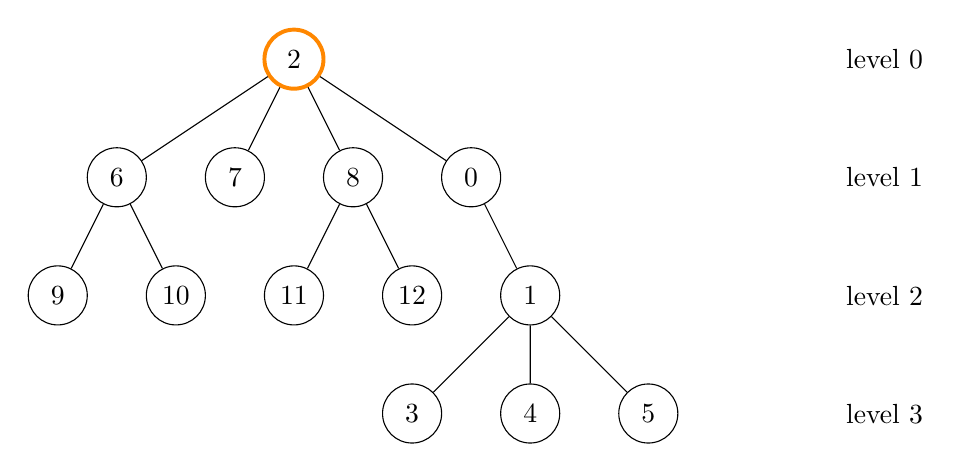
\begin{tikzpicture}[level/.style={sibling distance=15mm},  every node/.style={ minimum size=0.75cm}]
    \node [circle,draw=orange, line width = 0.5mm] (z){2}
        child {node [circle,draw] (a){6}
        child {node [circle,draw] (i) {9}}
        child {node [circle,draw] (j) {10}}
        }
        child {node [circle,draw] (b) {7}}
        child {node [circle,draw] (c) {8}
            child {node [circle,draw] (k) {11}}
            child {node [circle,draw] (l) {12}}
        }
        child {node [circle,draw] (d) {0}
            child {node (w) {} edge from parent[draw=none]}
            child {node [circle,draw] (e) {1}
                child {node [circle,draw] (f) {3}}
                child {node [circle,draw] (g) {4}}
                child {node [circle,draw] (h) {5}
                    child [grow=right] {node {} edge from parent[draw=none]
                        child [grow=right] {node (o) {level 3} edge from parent[draw=none]
                            child [grow=up] {node (p) {level 2} edge from parent[draw=none]
                                child [grow=up] {node (q) {level 1} edge from parent[draw=none]
                                    child [grow=up] {node {level 0} edge from parent[draw=none]}
                                }
                            }
                        }
                    }
                }
            }
        };
    \end{tikzpicture}
\end{frame}

\begin{frame}{Algorithm}
    \only<1>{In $\mathcal{O}(n)$, by Aho, Hopcroft and Ullman \cite{AhoHopcroftUllman}.}
    \only<2>{Assigned 0 to all leaves\\}
    \only<3>{Assign tuples to the vertices at level 2}
        \only<4>{Assign values to the distinct tuples, starting at 1, at level 2}
        \only<5>{Assign tuples to the vertices at level 1}
        \only<6>{Assign values to the distinct tuples}
        \only<7>{Assign tuples to the roots}
        \only<8>{Assign values to the root}
    \uncover<2>{\alert{Remark}: The orange indicates the final value of that node}
    \newcommand*\leafnodecolor{}
    \newcommand*\leaflinewidth{0.15mm}
    \newcommand*\leveltwonodecolor{}
    \newcommand*\leveltwolinewidth{0.15mm}
    \newcommand*\levelonenodecolor{}
    \newcommand*\levelonelinewidth{0.15mm}
    \newcommand*\rootnodecolor{}
    \newcommand*\rootlinewidth{0.15mm}
    \only<2->{\renewcommand*\leafnodecolor{orange}}
    \only<2->{\renewcommand*\leaflinewidth{0.5mm}}
    \only<4->{\renewcommand*\leveltwonodecolor{orange}}
    \only<4->{\renewcommand*\leveltwolinewidth{0.5mm}}
    \only<6->{\renewcommand*\levelonenodecolor{orange}}
    \only<6->{\renewcommand*\levelonelinewidth{0.5mm}}
    \only<8->{\renewcommand*\rootnodecolor{orange}}
    \only<8->{\renewcommand*\rootlinewidth{0.5mm}}
    \begin{center}
    \begin{tikzpicture}[level/.style={sibling distance=15mm},  every node/.style={ minimum size=0.75cm}]
    \node [circle,draw=\rootnodecolor, line width = \rootlinewidth] (z){\only<7>{(0,1,1,2)}\only<8>{1}}
        child {node [circle,draw=\levelonenodecolor, line width = \levelonelinewidth] (a){\only<5>{(0,0)}\only<6->{1}}
        child {node [circle,draw=\leafnodecolor, line width = \leaflinewidth] (i) {\only<2->0}}
        child {node [circle,draw=\leafnodecolor, line width = \leaflinewidth] (j) {\only<2->0}}
        }
        child {node [circle,draw=\leafnodecolor, line width = \leaflinewidth] (b) {\only<2->0}}
        child {node [circle, draw=\levelonenodecolor, line width = \levelonelinewidth] (c) {\only<5>{(0,0)}\only<6->{1}}
            child {node [circle,draw=\leafnodecolor, line width = \leaflinewidth] (k) {\only<2->0}}
            child {node [circle,draw=\leafnodecolor, line width = \leaflinewidth] (l) {\only<2->0}}
        }
        child {node [circle,draw=\levelonenodecolor, line width = \levelonelinewidth] (d) {\only<5>{(1)}\only<6->{2}}
            child {node (w) {} edge from parent[draw=none]}
            child {node [circle,draw=\leveltwonodecolor, line width = \leveltwolinewidth ] (e) {\only<3>{(0,0,0)}\only<4->{1}}
                child {node [circle,draw=\leafnodecolor, line width = \leaflinewidth] (f) {\only<2->0}}
                child {node [circle,draw=\leafnodecolor, line width = \leaflinewidth] (g) {\only<2->0}}
                child {node [circle,draw=\leafnodecolor, line width = \leaflinewidth] (h) {\only<2->0}
                    child [grow=right] {node {} edge from parent[draw=none]
                        child [grow=right] {node (o) {level 3} edge from parent[draw=none]
                            child [grow=up] {node (p) {level 2} edge from parent[draw=none]
                                child [grow=up] {node (q) {level 1} edge from parent[draw=none]
                                    child [grow=up] {node {level 0} edge from parent[draw=none]}
                                }
                            }
                        }
                    }
                }
            }
        };
    \end{tikzpicture}
    \end{center}
\end{frame}

\begin{frame}{Modular decomposition and trees}
\begin{itemize}
    \item Assign the same value to isomorphic modules, starting at the length of the vertices.
    \item Check if the modules in both graphs have the same tuples; otherwise their induced subtrees are different.
\end{itemize}
\end{frame}


\subsection{}
\againframe<11-12>{flow}

\subsection{Fast colour refinement and branching}

\pgfdeclarelayer{background}
\pgfdeclarelayer{foreground}
\pgfsetlayers{background,main,foreground}
\tikzstyle{vertex}=[circle, draw, inner sep=0pt, minimum size=15pt]
\newcommand{\vertex}{\node[vertex]}

% % Two simple graphs G and H are isomorphic if there exists a bijective mapping between them. Eg. $$f:V(G) \rightarrow V(H) st. \forall{u,v \in V(G): uv \in E(G) \leftrightarrow f(u)f(v) \in E(H)$$.
% % The fast colour refinement algorithm uses colours to define this mapping



% FIRST FLOW FRAME
\begin{frame}{Fast colour refinement and branching}
     \tikzstyle{box} = [draw, rectangle, text width=6em, text centered, fill=yellow!20, inner sep=3pt, minimum height=3em]
     \tikzstyle{cirkel} = [draw, circle, text width=5em, text centered, inner sep=0pt, minimum height=2em]
     \tikzstyle{test} = [diamond, draw, aspect=2, fill=orange!20, text width = 4em, minimum width = 4cm, minimum height = 2cm, inner sep=1pt, align=center]
    
     \begin{center}
      \begin{tikzpicture}[scale=0.8]
         \node[box] (init) at (0,3) {Initial colouring};
         \node[test] (fcr) at (0,0) {Use fast colour refinement};
         \node[cirkel, fill=red!20, opacity = 0.2](notiso) at (-7, 0){$G$ and $H$ are not isomorphic};
         \node[cirkel, fill=green!20, opacity = 0.2](iso) at (7,0){$G$ and $H$ are isomorphic};
        
         \path [->, thick] (init) edge node {} (fcr);
         \path [->, thick, opacity = 0.2] (fcr) edge node [text width=4em, below]{unbalanced colouring} (notiso);
         \path [->, thick, opacity = 0.2] (fcr) edge node [text width=4em, below]{bijective colouring} (iso);
%         \path [->,thick, opacity = 0.2] (fcr) edge [loop below] node {branch} (fcr);
     \end{tikzpicture}
     \end{center}
\end{frame}


% FAST COLOR REFINE EXAMPLE
\begin{frame}
% colours [1-red,2-orange,3-green, 4-blue, 5-yellow, 6-gray, 7-pink, 8-brown] 
\begin{itemize}
    \only<1>{
        \item Start with an initial colouring, eg. by degree
        \item Queue = [red, orange, green, blue]
    }
    \only<2>{
        \item Refine vertices on \textbf{amount of red neighbours}?
        \item Queue = [\sout{red}, orange, green, blue]
    }
    \only<3>{
        \item Refine orange vertices on \textbf{amount of orange neighbours}
        \item Queue = [\sout{orange}, green, blue]
    }
    \only<4>{
        \item Recolour orange vertices with 2 orange neighbours
        \item Queue = [green, blue] $\leftarrow$ \textcolor{orange}{orange}
    }
    \only<5>{
        \item Refine orange vertices on \textbf{amount of green neighbours}
        \item Queue = [\sout{green}, blue, orange]
    }
    \only<6>{
        \item Recolour orange vertices with no green neighbours
        \item Queue = [blue, orange] $\leftarrow$ \textcolor{gray}{gray}
    }
    \only<7->{
        \item Repeat these actions until the queue is empty
        \item Same colours $\rightarrow$ vertices map onto each other
    }
\end{itemize}

\quad

\begin{center}
    \begin{tikzpicture}[scale=.8]

    % GRAPH G
    \vertex[fill=blue!70](G0_0) at (-1,0){0};
    \vertex[fill=orange!70](G0_1) at (3,0){1};
    \vertex[fill=orange!70](G0_10) at (8,-1){10};
    \vertex[fill=orange!70](G0_11) at (0,0){11};
    \vertex[fill=orange!70](G0_12) at (4,0){12};
    \vertex[fill=orange!70](G0_13) at (2,0){13};
    \vertex[fill=red!70](G0_7) at (-2,0){7};
    \vertex[fill=orange!70](G0_14) at (1,-1){14};
    \vertex[fill=orange!70](G0_8) at (0,1){8};
    \vertex[fill=orange!70](G0_2) at (5,1){2};
    \vertex[fill=orange!70](G0_3) at (5,-1){3};
    \vertex[fill=orange!70](G0_4) at (5,0){4};
    \vertex[fill=orange!70](G0_5) at (2,-1){5};
    \vertex[fill=green!70](G0_6) at (8,0){6};
    \vertex[fill=orange!70](G0_9) at (1,0){9};
    
    \Edge(G0_0)(G0_7);
    \Edge(G0_14)(G0_0);
    \Edge(G0_0)(G0_11);
    \Edge(G0_0)(G0_8);
    \Edge(G0_12)(G0_1);
    \Edge(G0_1)(G0_13);
    \Edge(G0_2)(G0_8);
    \Edge(G0_6)(G0_2);
    \Edge(G0_10)(G0_3);
    \Edge(G0_5)(G0_3);
    \Edge(G0_12)(G0_4);
    \Edge(G0_4)(G0_6);
    \Edge(G0_10)(G0_6);
    \Edge(G0_9)(G0_11);
    \Edge(G0_14)(G0_5);
    \Edge(G0_13)(G0_9);

    % GRAPH H
    \vertex[fill=orange!70](G1_0)   at (0,-3){0};
    \vertex[fill=green!70](G1_13)   at (1,-3){13};
    \vertex[fill=orange!70](G1_1)   at (3,-4){1};
    \vertex[fill=orange!70](G1_10)  at (5,-6){10};
    \vertex[fill=orange!70](G1_11)  at (5,-3){11};
    \vertex[fill=blue!70](G1_12)    at (4,-3){12};
    \vertex[fill=orange!70](G1_14)  at (1,-5){14};
    \vertex[fill=orange!70](G1_2)   at (4,-5){2};
    \vertex[fill=orange!70](G1_3)   at (0,-5){3};
    \vertex[fill=orange!70](G1_4)   at (5,-5){4};
    \vertex[fill=orange!70](G1_5)   at (2,-3){5};
    \vertex[fill=red!70](G1_6)      at (4,-2){6};
    \vertex[fill=orange!70](G1_7)   at (2,-4){7};
    \vertex[fill=orange!70](G1_8)   at (3,-3){8};
    \vertex[fill=orange!70](G1_9)   at (0,-6){9};
    
    \Edge(G1_12)(G1_6);
    \Edge(G1_8)(G1_12);
    \Edge(G1_4)(G1_10);
    \Edge(G1_12)(G1_11);
    \Edge(G1_3)(G1_0);
    \Edge(G1_11)(G1_4);
    \Edge(G1_1)(G1_8);
    \Edge(G1_5)(G1_7);
    \Edge(G1_13)(G1_14);
    \Edge(G1_0)(G1_13);
    \Edge(G1_14)(G1_2);
    \Edge(G1_13)(G1_5);
    \Edge(G1_9)(G1_3);
    \Edge(G1_7)(G1_1);
    \Edge(G1_2)(G1_12);
    \Edge(G1_10)(G1_9);
    

    % % Refine on red?
    \only<2>{
    \begin{pgfonlayer}{background}
        \draw[rounded corners=1em,line width=1em,blue!20,cap=round]
            (-1.25,0.25) -- (-0.75,-0.25);
        \draw[rounded corners=1em,line width=1em,blue!20,cap=round]
            (3.75,-2.75) -- (4.25,-3.25);
    \end{pgfonlayer}
    }

    % % Refine orange on orange
    \only<3>{
    \begin{pgfonlayer}{background}
    % 1: 2,4,8,10,11,14    
        \draw[rounded corners=1em,line width=1em,orange!30,cap=round]
            (G0_10.center) -- (G0_4.west) --
            (G0_2.east) -- (G0_8.west) -- (G0_11.center) -- (G0_14.center);
    % 2: 1,3,5,9,12,13   
        \draw[rounded corners=1em,line width=1em,yellow!50,cap=round]
          (G0_5.center) -- (G0_9.west) -- (G0_13.center) -- (G0_1.center) --
          (G0_12.center) -- (G0_3.center);
    % 1: 0,2,5,8,11,14
        \draw[rounded corners=1em,line width=1em,orange!30,cap=round]
            (G1_14.center) --
            (G1_0.center) -- (1,-2) --
            (G1_5.center) -- (G1_8.north) --
            (G1_2.center) -- (G1_11.center);
    % 2: 1,3,4,7,9,10
        \draw[rounded corners=1em,line width=1em,yellow!50,cap=round]
            (G1_3.center) -- (G1_9.center) --
            (2,-6) -- (G1_7.center) --
            (G1_1.center) -- (3,-6) --
            (G1_10.center) -- (G1_4.center);
    \end{pgfonlayer}
    }
    \uncover<4->{
        \vertex[fill=yellow!70](G0_1) at (3,0){1};
        \vertex[fill=yellow!70](G0_12) at (4,0){12};
        \vertex[fill=yellow!70](G0_13) at (2,0){13};
        \vertex[fill=yellow!70](G0_3) at (5,-1){3};
        \vertex[fill=yellow!70](G0_5) at (2,-1){5};
        \vertex[fill=yellow!70](G0_9) at (1,0){9};
        
        \vertex[fill=yellow!70](G1_10) at (5,-6){10};   
        \vertex[fill=yellow!70](G1_1) at (3,-4){1};
        \vertex[fill=yellow!70](G1_4) at (5,-5){4};   
        \vertex[fill=yellow!70](G1_7) at (2,-4){7};   
        \vertex[fill=yellow!70](G1_3) at (0,-5){3};
        \vertex[fill=yellow!70](G1_9) at (0,-6){9};
    }
    

    % Refine orange on green
    \only<5>{
    \begin{pgfonlayer}{background}
     % 1: 2,4,10  
        \draw[rounded corners=1em,line width=1em,orange!30,cap=round]
            (G0_2.center) -- (G0_4.center) -- (G0_10.center);
     % 2: 8,11,14
        \draw[rounded corners=1em,line width=1em,gray!30,cap=round]
          (G0_8.center) -- (G0_11.center) -- (G0_14.center);
    % 1: 0,5,14
        \draw[rounded corners=1em,line width=1em,orange!30,cap=round]
            (G1_0.center) -- (G1_14.center) -- (G1_5.center);
     % 2: 2,8,11
        \draw[rounded corners=1em,line width=1em,gray!30,cap=round]
          (G1_8.center) -- (G1_2.center) -- (G1_11.center);
    \end{pgfonlayer}
    }
    \uncover<6->{
        \vertex[fill=gray!70](G0_11) at (0,0){11};
        \vertex[fill=gray!70](G0_14) at (1,-1){14};
        \vertex[fill=gray!70](G0_8) at (0,1){8};
        \vertex[fill=gray!70](G1_11) at (5,-3){11};
        \vertex[fill=gray!70](G1_2) at (4,-5){2};
        \vertex[fill=gray!70](G1_8) at (3,-3){8};
    }
    % REPEAT
    \uncover<7->{
        \vertex[fill=pink!70](G0_12) at (4,0){12};
        \vertex[fill=brown!70](G0_8) at (0,1){8};
        
        \vertex[fill=olive!70](G0_5) at (2,-1){5};
        \vertex[fill=violet!70](G0_3) at (5,-1){3};
        \vertex[fill=lime!70](G0_9) at (1,0){9};
        \vertex[fill=blue!30](G0_4) at (5,0){4};
        \vertex[fill=magenta!70](G0_13) at (2,0){13};
        \vertex[fill=orange!50!gray!20](G0_10) at (8,-1){10};
        \vertex[fill=green!30](G0_11) at (0,0){11};
        
        \vertex[fill=pink!70](G1_3) at (0,-5){3};
        \vertex[fill=brown!70](G1_2) at (4,-5){2};
        
        \vertex[fill=olive!70](G1_1) at (3,-4){1};
        \vertex[fill=violet!70](G1_7) at (2,-4){7};
        \vertex[fill=lime!70](G1_4) at (5,-5){4};
        \vertex[fill=blue!30](G1_0) at (0,-3){0};
        \vertex[fill=magenta!70](G1_10) at (5,-6){10};
        \vertex[fill=orange!50!gray!20](G1_5) at (2,-3){5};
        \vertex[fill=green!30](G1_11) at (5,-3){11};
    }

\end{tikzpicture}
\end{center}

\end{frame}

% FLOW PART 2
\begin{frame}{Colour refinement flow}
     \tikzstyle{box} = [draw, rectangle, text width=6em, text centered, fill=yellow!20, inner sep=3pt, minimum height=2em]
     \tikzstyle{cirkel} = [draw, circle, text width=5em, text centered, inner sep=0pt, minimum height=2em]
     \tikzstyle{test} = [diamond, draw, aspect=2, fill=orange!20, text width = 4em, minimum width = 4cm, minimum height = 2cm, inner sep=1pt, align=center]
     \begin{center}
     \begin{tikzpicture}[scale=0.8]
       \uncover<1>{\node[box] (init) at (0,3) {Initial colouring};}
       \node[test] (fcr) at (0,0) {Use fast colour refinement};
        \only<1>{\node[cirkel, fill=red!20](notiso) at (-7, 0){$G$ and $H$ are not isomorphic};
                       \node[cirkel, fill=green!20](iso) at (7,0){$G$ and $H$ are isomorphic};}
       \only<2>{\node[cirkel, fill=red!20, opacity = 0.2](notiso) at (-7, 0){$G$ and $H$ are not isomorphic};
                \node[cirkel, fill=green!20, opacity = 0.2](iso) at (7,0){$G$ and $H$ are isomorphic};}
       \uncover<1>{\path [->, thick] (init) edge node {} (fcr);}
       \only<1>{\path [->, thick] (fcr) edge node [text width=4em, below]{unbalanced colouring} (notiso);
                \path [->, thick] (fcr) edge node [text width=4em, below]{bijective colouring} (iso);}
       \only<2>{\path [->, thick, opacity = 0.2] (fcr) edge node [text width=4em, below]{unbalanced colouring} (notiso);
                \path [->, thick, opacity = 0.2] (fcr) edge node [text width=4em, below]{bijective colouring} (iso);}
       \uncover<2->{\path [->,thick] (fcr) edge [loop below] node {branch} (fcr);}
     \end{tikzpicture}
     \end{center}
\end{frame}
% EXAMPLE BRANCHING
\begin{frame}{Branching}
Sometimes fast colour refinement results in a balanced non-bijective colouring.
\begin{itemize}
    \item There are multiple possible mappings
    \uncover<2->{\item Pick a colour class with at least 4 vertices}
    \uncover<3->{\item Pick a vertex from G (eg. G0)}
    \uncover<4->{\item Branch on vertices of H}
\end{itemize}

\begin{center}\begin{tikzpicture}[scale=0.8]
    \uncover<1-3>{
        \node(G) at (-2,0){G:};
        \node(H) at (-2,-2){H:};
    }

    \vertex[fill=blue!70](G0_0) at (0,0){0};
    \vertex[fill=orange!70](G0_1) at (1,0){1};
    \vertex[fill=green!70](G0_2) at (2,0){2};
    \vertex[fill=yellow!70](G0_3) at (2,-1){3};
    \vertex[fill=green!70](G0_4) at (3,0){4};
    \vertex[fill=orange!70](G0_5) at (4,0){5};
    \vertex[fill=blue!70](G0_6) at (5,0){6};
    \Edge(G0_1)(G0_0);
    \Edge(G0_2)(G0_1);
    \Edge(G0_3)(G0_2);
    \Edge(G0_4)(G0_3);
    \Edge(G0_4)(G0_2);
    \Edge(G0_5)(G0_4);
    \Edge(G0_6)(G0_5);
    
    \uncover<1-3>{
        \vertex[fill=green!70](G2_0) at (3,-2){0};
        \vertex[fill=blue!70](G2_1) at (0,-2){1};
        \vertex[fill=blue!70](G2_2) at (4,-3){2};
        \vertex[fill=orange!70](G2_3) at (1,-2){3};
        \vertex[fill=yellow!70](G2_4) at (2,-3){4};
        \vertex[fill=green!70](G2_5) at (2,-2){5};
        \vertex[fill=orange!70](G2_6) at (3,-3){6};
        \Edge(G2_3)(G2_1);
        \Edge(G2_5)(G2_3);
        \Edge(G2_5)(G2_0);
        \Edge(G2_4)(G2_0);
        \Edge(G2_5)(G2_4);
        \Edge(G2_6)(G2_0);
        \Edge(G2_6)(G2_2);
    }
   
    \only<2>{
        \begin{pgfonlayer}{background}
            \draw[rounded corners=1em,line width=1em,blue!20,cap=round]
                (G0_0.center) -- (G2_1.center) --
                (0,-4) -- (4,-4) --
                (G2_2.center) -- (G0_6.center);
        \end{pgfonlayer}
    }
    \uncover<3->{
        \vertex[fill=blue!30](G0_0) at (0,0){0};
    }
    \uncover<4->{
        \node(G) at (-4,0){G:};
        \node(H) at (-4,-3){H:};
    
      \vertex[fill=green!70](G2_0) at (0,-3){0};
      \vertex[fill=blue!30](G2_1) at (-3,-3){1};
      \vertex[fill=blue!70](G2_2) at (1,-4){2};
      \vertex[fill=orange!70](G2_3) at (-2,-3){3};
      \vertex[fill=yellow!70](G2_4) at (-1,-4){4};
      \vertex[fill=green!70](G2_5) at (-1,-3){5};
      \vertex[fill=orange!70](G2_6) at (0,-4){6};
      \Edge(G2_3)(G2_1);
      \Edge(G2_5)(G2_3);
      \Edge(G2_5)(G2_0);
      \Edge(G2_4)(G2_0);
      \Edge(G2_5)(G2_4);
      \Edge(G2_6)(G2_0);
      \Edge(G2_6)(G2_2);
       
      \vertex[fill=green!70](2_0) at (6,-3){0};
      \vertex[fill=blue!70](2_1) at (3,-3){1};
      \vertex[fill=blue!30](2_2) at (7,-4){2};
      \vertex[fill=orange!70](2_3) at (4,-3){3};
      \vertex[fill=yellow!70](2_4) at (5,-4){4};
      \vertex[fill=green!70](2_5) at (5,-3){5};
      \vertex[fill=orange!70](2_6) at (6,-4){6};
      \Edge(2_3)(2_1);
      \Edge(2_5)(2_3);
      \Edge(2_5)(2_0);
      \Edge(2_4)(2_0);
      \Edge(2_5)(2_4);
      \Edge(2_6)(2_0);
      \Edge(2_6)(2_2);
       
      \path[->, thick] (1,-1.5) edge node [above left, midway]{pick H1 (branch1)} (0.5,-2);
      \path[->, thick] (3,-1.5) edge node[above right, midway] {pick H2 (branch2)} (3.5,-2);
    }
   
\end{tikzpicture}
\end{center}
\end{frame}
\begin{frame}{Colour refinement flow}
     \tikzstyle{box} = [draw, rectangle, text width=6em, text centered, fill=yellow!20, inner sep=3pt, minimum height=3em]
          \tikzstyle{cirkel} = [draw, circle, text width=5em, text centered, inner sep=0pt, minimum height=2em]
          \tikzstyle{test} = [diamond, draw, aspect=2, fill=orange!20, text width = 4em, minimum width = 4cm, minimum height = 2cm, inner sep=1pt, align=center]

          \begin{center}
           \begin{tikzpicture}[scale=0.8]
              \node[box] (init) at (0,3) {Initial colouring};
              \node[test] (fcr) at (0,0) {Use fast colour refinement};
              \node[cirkel, fill=red!20](notiso) at (-7, 0){$G$ and $H$ are not isomorphic};
              \node[cirkel, fill=green!20](iso) at (7,0){$G$ and $H$ are isomorphic};

              \path [->, thick] (init) edge node {} (fcr);
              \path [->, thick] (fcr) edge node [text width=4em, below]{unbalanced colouring} (notiso);
              \path [->, thick] (fcr) edge node [text width=4em, below]{bijective colouring} (iso);
              \path [->,thick] (fcr) edge [loop below] node {branch} (fcr);
          \end{tikzpicture}
          \end{center}
\end{frame}

\subsection{}
\againframe<14>{flow}
\subsection{}
\againframe<3>{processing-overview}
\subsection{Number of automorphisms}
% \begin{frame}{Counting Automorphisms}

% Brute force approach:
% \begin{enumerate}
%     \item Compute all leaves of the tree
%     \item Count leaves that result in a unique permutation
% \end{enumerate}

% Idea: don't determine each possible permutation, but use generating sets
% \end{frame}

\begin{frame}{Counting automorphisms}
    \begin{center}
        \begin{tikzpicture}
    \renewcommand*{\VertexLineWidth}{1.6pt}
    \renewcommand*{\VertexLineColor}{blue}
    \Vertex[x=1, y=0]{4}
    \Vertex[x=0, y=0]{1}
    \renewcommand*{\VertexLineColor}{red}
    \Vertex[x=-1, y=0]{0}
    \Vertex[x=2, y=0]{5}
    \renewcommand*{\VertexLineColor}{green}
    \Vertex[x=0.5, y=1]{2}
    \Vertex[x=0.5, y=-1]{3}
    \Edge(0)(1)
    \Edge(1)(2)
    \Edge(1)(3)
    \Edge(2)(4)
    \Edge(3)(4)
    \Edge(4)(5)
\end{tikzpicture}

        \begin{forest}
    leaf/.style={font=\bfseries}
    [{()}, delay={where content={}{shape=coordinate}{}}
        [{()}, edge label={node[midway,left,font=\scriptsize]{1$\rightarrow$1}}
            [{()},edge label={node[midway,left,font=\scriptsize]{2$\rightarrow$2}}
            ]   
            [{(2,3)},edge label={node[midway,right,font=\scriptsize]{2$\rightarrow$3}}
            ]
        ]
        [{(1,4)(0,5)},edge label={node[midway,right,font=\scriptsize]{1$\rightarrow$4}}
            [{(1,4)(0,5)},edge label={node[midway,left,font=\scriptsize]{2$\rightarrow$2}}
            ]
            [{(1,4)(0,5)(2,3)},edge label={node[midway,right,font=\scriptsize]{2$\rightarrow$3}}
            ]
        ]
    ]
\end{forest}

    \end{center}
\end{frame}

\begin{frame}{Automorphism groups}
    \uncover<1->{
        \begin{itemize}
            \item number automorphisms is a group% under composition
            \item generating set: subgroup of a group which generates all elements of the group
            \item generating set can be small for large groups
            % \item in many cases efficiently calculated
        \end{itemize}
    }
    \uncover<2->{
        \begin{center}
        \scalebox{0.7}{
            \begin{tikzpicture}
    \renewcommand*{\VertexLineWidth}{1.6pt}
    \renewcommand*{\VertexLineColor}{blue}
    \Vertex[x=1, y=0]{4}
    \Vertex[x=0, y=0]{1}
    \renewcommand*{\VertexLineColor}{red}
    \Vertex[x=-1, y=0]{0}
    \Vertex[x=2, y=0]{5}
    \renewcommand*{\VertexLineColor}{green}
    \Vertex[x=0.5, y=1]{2}
    \Vertex[x=0.5, y=-1]{3}
    \Edge(0)(1)
    \Edge(1)(2)
    \Edge(1)(3)
    \Edge(2)(4)
    \Edge(3)(4)
    \Edge(4)(5)
\end{tikzpicture}

        }
        \input{num_auto_files/tree_example2.tex}
        \end{center}
    }
\end{frame}

\begin{frame}{Tree pruning}
\scalebox{0.7}{
    \begin{tikzpicture}
    \renewcommand*{\VertexLineWidth}{1.6pt}
    \renewcommand*{\VertexLineColor}{blue}
    \Vertex[x=-2, y=0]{0}
    \Vertex[x=2, y=0]{8}
    \renewcommand*{\VertexLineColor}{green}
    \Vertex[x=-1, y=0]{3}
    \Vertex[x=1, y=0]{5}
    \renewcommand*{\VertexLineColor}{red}
    \Vertex[x=0, y=0]{4}
    \Vertex[x=-1.5, y=1]{1}
    \Vertex[x=-1.5, y=-1]{2}
    \Vertex[x=1.5, y=1]{6}
    \Vertex[x=1.5, y=-1]{7}
    \Edge(0)(1)
    \Edge(0)(2)
    \Edge(0)(3)
    \Edge(1)(3)
    \Edge(2)(3)
    \Edge(3)(4)
    \Edge(4)(5)
    \Edge(5)(6)
    \Edge(5)(7)
    \Edge(5)(8)
    \Edge(6)(8)
    \Edge(7)(8)
\end{tikzpicture}

}
\scalebox{0.9}{
    \begin{forest}
    leaf/.style={font=\bfseries}
    [{()}, delay={where content={}{shape=coordinate}{}}
        [{()},edge=orange, edge label={node[midway,left,font=\scriptsize]{0$\rightarrow$0}}
            [{()},edge=orange,edge label={node[midway,left,font=\scriptsize]{3$\rightarrow$3}}
                [{()},edge=orange,edge label={node[midway,left,font=\scriptsize]{1$\rightarrow$1}}
                    [{()},leaf, edge label={node[midway,left,font=\scriptsize]{6$\rightarrow$6}}]
                    [{\textcolor{orange}{(6,7)}},leaf,edge=orange,edge label={node[midway,right,font=\scriptsize]{6$\rightarrow$7}}]
                ]
                [{(1,2)},edge=orange,edge label={node[midway,right,font=\scriptsize]{1$\rightarrow$2}}
                    [{\textcolor{orange}{(1,2)}},leaf,edge=orange,edge label={node[midway,left,font=\scriptsize]{6$\rightarrow$6}}]
                    [{(1,2)(6,7)},leaf,edge label={node[midway,right,font=\scriptsize]{6$\rightarrow$7}}]
                ]
            ]   
            [{(3,5)},edge label={node[midway,right,font=\scriptsize]{3$\rightarrow$5}}
                [, edge=dashed
                    [-,leaf, edge=dashed]
                ]
            ]
        ]
        [{(0,8)},edge=orange,edge label={node[midway,right,font=\scriptsize]{0$\rightarrow$8}}
            [{(0,8)},edge label={node[midway,left,font=\scriptsize]{3$\rightarrow$3}}
                [, edge=dashed
                    [-,leaf, edge=dashed]
                ]
            ]
            [{(0,8)(3,5)},edge=orange,edge label={node[midway,right,font=\scriptsize]{3$\rightarrow$5}}
                [{(0,8)(3,5)(1,6)(2,7)},edge=orange,edge label={node[midway,right,font=\scriptsize]{1$\rightarrow$6}}
                    [{\textcolor{orange}{(0,8)(3,5)}\\\textcolor{orange}{(1,6,2,7)}},leaf,align=center,edge=orange,edge label={node[midway,left,font=\scriptsize]{6$\rightarrow$2}}]
                    [{(0,8)(3,5)\\(1,6)(2,7)},leaf,align=center,edge label={node[midway,left,font=\scriptsize]{6$\rightarrow$1}}]
                ]
                [{(0,8)(3,5)(1,7)(2,6)},edge label={node[midway,right,font=\scriptsize]{1$\rightarrow$7}}
                    [{(0,8)(3,5)\\(1,7,2,6)},leaf,align=center,edge label={node[midway,left,font=\scriptsize]{6$\rightarrow$1}}]
                    [{(0,8)(3,5)\\(1,7)(2,6)},leaf,align=center,edge label={node[midway,right,font=\scriptsize]{6$\rightarrow$2}}]
                ]
            ]
        ]
    ]
\end{forest}
}
\end{frame}

\begin{frame}{Generating set}
    \begin{center}
         \textcolor{orange}{[(6,7), (1,2), (0,8)(3,5)(1,6,2,7)]}
    \end{center}
     \begin{itemize}
        \item order: number of automorphisms
        \item non-trivial mapping: mapping of a node to another node
        \item orbit: all possible mappings of a node
        \item stabilizer: permutations in the set where a node maps to itself
    \end{itemize}
\end{frame}

\begin{frame}{Compute number of automorphisms}
    \begin{center}
    \scalebox{0.7}{
        \begin{tikzpicture}
    \renewcommand*{\VertexLineWidth}{1.6pt}
    \renewcommand*{\VertexLineColor}{blue}
    \Vertex[x=-2, y=0]{0}
    \Vertex[x=2, y=0]{8}
    \renewcommand*{\VertexLineColor}{green}
    \Vertex[x=-1, y=0]{3}
    \Vertex[x=1, y=0]{5}
    \renewcommand*{\VertexLineColor}{red}
    \Vertex[x=0, y=0]{4}
    \Vertex[x=-1.5, y=1]{1}
    \Vertex[x=-1.5, y=-1]{2}
    \Vertex[x=1.5, y=1]{6}
    \Vertex[x=1.5, y=-1]{7}
    \Edge(0)(1)
    \Edge(0)(2)
    \Edge(0)(3)
    \Edge(1)(3)
    \Edge(2)(3)
    \Edge(3)(4)
    \Edge(4)(5)
    \Edge(5)(6)
    \Edge(5)(7)
    \Edge(5)(8)
    \Edge(6)(8)
    \Edge(7)(8)
\end{tikzpicture}

    }
    \end{center}
    \begin{table}[]
        \centering
        \label{my-label}
        \begin{tabular}{lll}
        generating set      & {[}(6,7),(1,2),(0,8)(1,6,2,7)(3,5){]}             & \uncover<3->{{[}(6,7){]}} \\
        non-trivial mapping & 1                                                 & \uncover<3->{6}           \\
        orbit               & (1,2,6,7)                                         & \uncover<3->{(6,7)}       \\
        stabilizer          & {[}(6,7){]}                                       & \uncover<3->{-}           \\
        order               & length(orbit) $\times$ order of {[}(6,7){]}       & \uncover<3->{length(orbit)}           \\
                            & \uncover<2->{= 4 $\times$ order of {[}(6,7){]}}   & \uncover<3->{= 2}
        \end{tabular}
    \end{table}
    \uncover<3>{
        \begin{center}
            number of automorphisms = 8
        \end{center}
    }
\end{frame}
\subsection{}
\againframe<4>{processing-overview}

\section{Results}
% Gegenereerd met tablesgenerator.com

% Maak tabellen passend met:
% \adjustbox{max height=\dimexpr\textheight-\dy\relax,max width=\textwidth}{
% ...
% }

\begin{frame}{Results of the basic graphs}
\begin{table}[]
\centering
\adjustbox{max height=\dimexpr\textheight-\dy\relax,max width=\textwidth}{
\begin{tabular}{@{}lrrrrrrr@{}}
\toprule
\begin{tabular}[c]{@{}l@{}}file\\ name\end{tabular} & \begin{tabular}[c]{@{}r@{}}number\\ of graphs\end{tabular} & \begin{tabular}[c]{@{}r@{}}graph\\ order\end{tabular} & \begin{tabular}[c]{@{}r@{}}graph\\ size\end{tabular} & \begin{tabular}[c]{@{}r@{}}modular decom-\\ position factor\end{tabular} & \begin{tabular}[c]{@{}r@{}}isomorphic\\ graphs\end{tabular} & \begin{tabular}[c]{@{}r@{}}number of\\ automorphisms\end{tabular} & \begin{tabular}[c]{@{}r@{}}time to solve\\ (sec)\end{tabular} \\ \midrule
basicAut1.gr & 1 & 35 & 34 & 576 & -- & 2304 & 0.037 \\ \midrule
basicAut2.gr & 1 & 69 & 96 & 1 & -- & 128 & 1.554 \\ \midrule
basicGI1.grl & 4 & 147 & 857 & 1 & \begin{tabular}[c]{@{}r@{}}$[0, 2]$\\ $[1, 3]$\end{tabular} & -- & 10.678 \\ \midrule
basicGI2.grl & 4 & 40 & 60 & 1 & \begin{tabular}[c]{@{}r@{}}$[0, 2]$\\ $[1, 3]$\end{tabular} & -- & 6.179 \\ \midrule
basicGI3.grl & 7 & 32 & 80 & 1 & \begin{tabular}[c]{@{}r@{}}$[0, 2, 6]$\\ $[1, 3, 4, 5]$\end{tabular} & -- & 1.813 \\ \midrule
basicGIAut.grl & 9 & 40 & 75 & 1 & \begin{tabular}[c]{@{}r@{}}$[0, 5, 7]$\\ $[1, 6]$\\ $[2, 3]$\\ $[4, 8]$\end{tabular} & \begin{tabular}[c]{@{}r@{}}10\\ 20\\ 20\\ 10\end{tabular} & 3.719 \\ \bottomrule
\end{tabular}
}
\end{table}
\end{frame}

\begin{frame}{Results of the bonus graph isomorphism problems}
\begin{table}[]
\centering
\adjustbox{max height=\dimexpr\textheight-\dy\relax,max width=\textwidth}{
\begin{tabular}{@{}lrrrrrr@{}}
\toprule
\begin{tabular}[c]{@{}l@{}}file\\ nr\end{tabular} & \begin{tabular}[c]{@{}r@{}}number\\ of graphs\end{tabular} & \begin{tabular}[c]{@{}r@{}}graph\\ order\end{tabular} & \begin{tabular}[c]{@{}r@{}}graph\\ size\end{tabular} & \begin{tabular}[c]{@{}r@{}}modular decom-\\ position factor\end{tabular} & \begin{tabular}[c]{@{}r@{}}isomorphic\\ graphs\end{tabular} & \begin{tabular}[c]{@{}r@{}}time to solve\\ (min:sec)\end{tabular} \\ \midrule
\textbf<2>{1} & \textbf<2>{8} & \textbf<2>{52} & \textbf<2>{\{762, 858\}} & \begin{tabular}[c]{@{}r@{}}\textbf<2>{67108864}\\ \textbf<2>{4403012567040000}\\ \textbf<2>{543581798400}\\ \textbf<2>{4403012567040000}\end{tabular} & \begin{tabular}[c]{@{}r@{}}\textbf<2>{[0, 7]}\\ \textbf<2>{[1, 6]}\\ \textbf<2>{[2, 4]}\\ \textbf<2>{[3, 5]}\end{tabular} & \textbf<2>{0.9} \\ \midrule
\textbf<3>{2} & \textbf<3>{12} & \textbf<3>{64} & \textbf<3>{204} & \begin{tabular}[c]{@{}r@{}}\textbf<3>{86973087744}\\ \textbf<3>{67108864}\\ \textbf<3>{5706304286883840000}\\ \textbf<3>{4403012567040000}\\ \textbf<3>{704482010726400}\\ \textbf<3>{5706304286883840000}\end{tabular} & \begin{tabular}[c]{@{}r@{}}\textbf<3>{[0, 3]}\\ \textbf<3>{[1, 4]}\\ \textbf<3>{[2 ,9]}\\ \textbf<3>{[5, 10]}\\ \textbf<3>{[6, 7]}\\ \textbf<3>{[8, 11]}\end{tabular} & \textbf<3>{0.4} \\ \midrule
3 & 4 & 627 & 6777 & 1 & $[0, 3]$, $[1, 2]$ & 15:46.6 \\ \midrule
4 & 6 & 80 & 120 & 1 & $[0, 2, 3, 4]$, $[1, 5]$ & 6:27.5 \\ \midrule
5 & 8 & 300 & 300 & 1 & $[0, 2]$, $[1, 3]$, $[4, 6]$, $[5, 7]$ & 1.5 \\ \bottomrule
\end{tabular}
}
\end{table}
\end{frame}

\begin{frame}{Results of the bonus automorphism problems}
\begin{table}[]
\centering
\adjustbox{max height=\dimexpr\textheight-\dy\relax,max width=\textwidth}{
\begin{tabular}{@{}lrrrrrr@{}}
\toprule
\begin{tabular}[c]{@{}l@{}}file\\ nr\end{tabular} & \begin{tabular}[c]{@{}r@{}}number\\ of graphs\end{tabular} & \begin{tabular}[c]{@{}r@{}}graph\\ order\end{tabular} & \begin{tabular}[c]{@{}r@{}}graph\\ size\end{tabular} & \begin{tabular}[c]{@{}r@{}}modular decom-\\ position factor\end{tabular} & \begin{tabular}[c]{@{}r@{}}number of\\ automorphisms\end{tabular} & \begin{tabular}[c]{@{}r@{}}time to solve\\ (min:sec)\end{tabular} \\ \midrule
\textbf<2>{1} & \textbf<2>{1} & \textbf<2>{995} & \textbf<2>{994} & \textbf<2>{1} & \textbf<2>{3538944} & \textbf<2>{27:36.5} \\ \midrule
\textbf<2>{2} & \textbf<2>{1} & \textbf<2>{181} & \textbf<2>{180} & \textbf<2>{13589544960000} & \textbf<2>{305267893261020841472415498240000} & \textbf<2>{5:02.7} \\ \midrule
\textbf<3>{3} & \textbf<3>{4} & \textbf<3>{36} & \textbf<3>{126} & \textbf<3>{262144} & \begin{tabular}[c]{@{}r@{}}\textbf<3>{5435817984}\\ \textbf<3>{32614907904}\\ \textbf<3>{32614907904}\\ \textbf<3>{5435817984}\end{tabular} & \textbf<3>{2.4} \\ \midrule
\textbf<4>{4} & \textbf<4>{3} & \textbf<4>{240} & \textbf<4>{480} & \textbf<4>{1} & \begin{tabular}[c]{@{}r@{}}\textbf<4>{12779520}\\ \textbf<4>{17031168}\\ \textbf<4>{16220160}\end{tabular} & \textbf<4>{32:50.6} \\ \midrule
5 & 3 & 86 & 165 & \begin{tabular}[c]{@{}r@{}}16\\ 4\\ 6\end{tabular} & \begin{tabular}[c]{@{}r@{}}9277129359360\\ 1307993702400\\ 2231764254720\end{tabular} & 2:44.3 \\ \midrule
\uncover<5->{- & 1 & 298 & 297 & 210357201231685877760000 & \begin{tabular}[c]{@{}r@{}}9587292865845886180...\\ 9541639114720040295...\\ 52885047052206080000\end{tabular} & 53:42.5 \\ \bottomrule}
\end{tabular}
}
\end{table}
\end{frame}

\section*{Conclusion and Discussion}

\begin{frame}{Conclusion}
    \begin{itemize}
        \item All basic instances were successfully solved
        \item GI-problem could efficiently be solved for:
        \begin{itemize}
            \item graphs were the complement is smaller
            \item trees
            \item graphs with modules
            \item disconnected graphs
        \end{itemize}
        \item Number of automorphisms had only a smart algorithm for graphs with modules
        \item Bug in the detection of isomorphic graphs with disconnected components
    \end{itemize}
\end{frame}

\begin{frame}{Possible improvements}
  \begin{itemize}
    \item Optimisation for fast colour refinement after branching
    \item Use smart branching
    \item Use efficient algorithms for different types of graphs for the number of automorphisms
    % \item Smart tree-graph handling while counting automorphisms
    % \item Use disconnected graphs to increase speed in counting automorphisms
  \end{itemize}
\end{frame}

\begin{frame}{Reflection}
  \begin{itemize}
    \item Development of different good ideas in parallel does not guarantee good results
    \item However, the team effort ultimately resulted in a successful integration
  \end{itemize}
\end{frame}

\section*{Appendix}
\subsection*{Bibliography}
\begin{frame}{Bibliography}
    
  \begin{thebibliography}{10}
    
  \beamertemplatebookbibitems
  % Start with overview books.

  \bibitem{AhoHopcroftUllman}
    A. V. Aho, J. E. Hopcroft, and J. D. Ullman. 
    \newblock {\em The Design and Analysis of Computer Algorithms}.
    \newblock Addison-Wesley, 1974.
    
  \beamertemplatearticlebibitems
  % Followed by interesting articles. Keep the list short. 
  \bibitem{bonamy2010small}
    Marthe Bonamy.
    \newblock A small report on graph and tree isomorphism.
    \newblock 2010.
    
  \end{thebibliography}
\end{frame}

\subsection*{Results after improvements}
\begin{frame}{Results of the basic graphs - improved}
\begin{table}[]
\centering
\adjustbox{max height=\dimexpr\textheight-\dy\relax,max width=\textwidth}{
\begin{tabular}{@{}lrrrrrrrrrr@{}}
\toprule
\multirow{2}{*}{\begin{tabular}[c]{@{}l@{}}file\\ name\end{tabular}} & \multirow{2}{*}{\begin{tabular}[c]{@{}r@{}}number\\ of graphs\end{tabular}} & \multirow{2}{*}{\begin{tabular}[c]{@{}r@{}}graph\\ order\end{tabular}} & \multirow{2}{*}{\begin{tabular}[c]{@{}r@{}}graph\\ size\end{tabular}} & \multirow{2}{*}{\begin{tabular}[c]{@{}r@{}}MD\\ factor\end{tabular}} & \multicolumn{2}{c}{after MD} & \multirow{2}{*}{\begin{tabular}[c]{@{}r@{}}isomorphic\\ graphs\end{tabular}} & \multirow{2}{*}{\begin{tabular}[c]{@{}r@{}}number of\\ automorphisms\end{tabular}} & \multirow{2}{*}{\begin{tabular}[c]{@{}r@{}}time to solve\\ (sec)\end{tabular}} & \multirow{2}{*}{\begin{tabular}[c]{@{}r@{}}time to solve\\ improved (sec)\end{tabular}} \\
 &  &  &  &  & order & size &  &  &  &  \\ \midrule
basicAut1.gr & 1 & 35 & 34 & 576 & 27 & 26 & -- & 2304 & 0.037 & 0.016 \\ \midrule
basicAut2.gr & 1 & 69 & 96 & 1 & - & - & -- & 128 & 1.554 & 0.146 \\ \midrule
basicGI1.grl & 4 & 147 & 857 & 1 & \begin{tabular}[c]{@{}r@{}}-\\ -\end{tabular} & \begin{tabular}[c]{@{}r@{}}-\\ -\end{tabular} & \begin{tabular}[c]{@{}r@{}}$[0, 2]$\\ $[1, 3]$\end{tabular} & -- & 10.678 & 1.843 \\ \midrule
basicGI2.grl & 4 & 40 & 60 & 1 & \begin{tabular}[c]{@{}r@{}}-\\ -\end{tabular} & \begin{tabular}[c]{@{}r@{}}-\\ -\end{tabular} & \begin{tabular}[c]{@{}r@{}}$[0, 2]$\\ $[1, 3]$\end{tabular} & -- & 6.179 & 3.550 \\ \midrule
basicGI3.grl & 7 & 32 & 80 & 1 & \begin{tabular}[c]{@{}r@{}}-\\ -\end{tabular} & \begin{tabular}[c]{@{}r@{}}-\\ -\end{tabular} & \begin{tabular}[c]{@{}r@{}}$[0, 2, 6]$\\ $[1, 3, 4, 5]$\end{tabular} & -- & 1.813 & 1.700 \\ \midrule
basicGIAut.grl & 9 & 40 & 75 & 1 & \begin{tabular}[c]{@{}r@{}}-\\ -\\ -\\ -\end{tabular} & \begin{tabular}[c]{@{}r@{}}-\\ -\\ -\\ -\end{tabular} & \begin{tabular}[c]{@{}r@{}}$[0, 5, 7]$\\ $[1, 6]$\\ $[2, 3]$\\ $[4, 8]$\end{tabular} & \begin{tabular}[c]{@{}r@{}}10\\ 20\\ 20\\ 10\end{tabular} & 3.719 & 2.573 \\ \bottomrule
\end{tabular}
}
\end{table}
\end{frame}

\begin{frame}{Results of the bonus graph isomorphism problems - improved}
\begin{table}[]
\centering
\adjustbox{max height=\dimexpr\textheight-\dy\relax,max width=\textwidth}{
\begin{tabular}{@{}lrrrrrrrrr@{}}
\toprule
\multirow{2}{*}{\begin{tabular}[c]{@{}l@{}}file\\ nr\end{tabular}} & \multirow{2}{*}{\begin{tabular}[c]{@{}r@{}}number\\ of graphs\end{tabular}} & \multirow{2}{*}{\begin{tabular}[c]{@{}r@{}}graph\\ order\end{tabular}} & \multirow{2}{*}{\begin{tabular}[c]{@{}r@{}}graph\\ size\end{tabular}} & \multirow{2}{*}{\begin{tabular}[c]{@{}r@{}}MD\\ factor\end{tabular}} & \multicolumn{2}{c}{after MD} & \multirow{2}{*}{\begin{tabular}[c]{@{}r@{}}isomorphic\\ graphs\end{tabular}} & \multirow{2}{*}{\begin{tabular}[c]{@{}r@{}}time to solve\\ (min:sec)\end{tabular}} & \multirow{2}{*}{\begin{tabular}[c]{@{}r@{}}time to solve\\ improved (min:sec)\end{tabular}} \\
 &  &  &  &  & order & size &  &  &  \\ \midrule
1 & 8 & 52 & $\{762, 858\}$ & \begin{tabular}[c]{@{}r@{}}67108864\\ 4403012567040000\\ 543581798400\\ 4403012567040000\end{tabular} & \begin{tabular}[c]{@{}r@{}}26\\ 18\\ 22\\ 18\end{tabular} & \begin{tabular}[c]{@{}r@{}}18\\ 50$^*$\\ 143\\ 103\end{tabular} & \begin{tabular}[c]{@{}r@{}}$[0, 7]$\\ $[1, 6]$\\ $[2, 4]$\\ $[3, 5]$\end{tabular} & 0.928 & 0.611 \\ \midrule
2 & 12 & 64 & 204 & \begin{tabular}[c]{@{}r@{}}86973087744\\ 67108864\\ 5706304286883840000\\ 4403012567040000\\ 704482010726400\\ 5706304286883840000\end{tabular} & \begin{tabular}[c]{@{}r@{}}30\\ 38\\ 22\\ 30\\ 26\\ 22\end{tabular} & \begin{tabular}[c]{@{}r@{}}45\\ 61\\ 25\\ 41\\ 33\\ 25\end{tabular} & \begin{tabular}[c]{@{}r@{}}$[0, 3]$\\ $[1, 4]$\\ $[2 ,9]$\\ $[5, 10]$\\ $[6, 7]$\\ $[8, 11]$\end{tabular} & 0.438 & 0.305 \\ \midrule
3 & 4 & 627 & 6777 & 1 & - & - & $[0, 3]$, $[1, 2]$ & 15:46.585 & 58.621 \\ \midrule
4 & 6 & 80 & 120 & 1 & - & - & $[0, 2, 3, 4]$, $[1, 5]$ & 6:27.488 & 3:01:330 \\ \midrule
5 & 8 & 300 & 300 & 1 & - & - & $[0, 2]$, $[1, 3]$, $[4, 6]$, $[5, 7]$ & 1.549 & 1.559 \\ \bottomrule
\end{tabular}
}
\end{table}
\end{frame}

\begin{frame}{Results of the bonus automorphism problems - improved}
\begin{table}[]
\centering
\adjustbox{max height=\dimexpr\textheight-\dy\relax,max width=\textwidth}{
\begin{tabular}{@{}lrrrrrrrrr@{}}
\toprule
\multirow{2}{*}{\begin{tabular}[c]{@{}l@{}}file\\ nr\end{tabular}} & \multirow{2}{*}{\begin{tabular}[c]{@{}r@{}}number\\ of graphs\end{tabular}} & \multirow{2}{*}{\begin{tabular}[c]{@{}r@{}}graph\\ order\end{tabular}} & \multirow{2}{*}{\begin{tabular}[c]{@{}r@{}}graph\\ size\end{tabular}} & \multirow{2}{*}{\begin{tabular}[c]{@{}r@{}}MD\\ factor\end{tabular}} & \multicolumn{2}{c}{after MD} & \multirow{2}{*}{\begin{tabular}[c]{@{}r@{}}number of\\ automorphisms\end{tabular}} & \multirow{2}{*}{\begin{tabular}[c]{@{}r@{}}time to solve\\ (min:sec)\end{tabular}} & \multirow{2}{*}{\begin{tabular}[c]{@{}r@{}}time to solve\\ improved (min:sec)\end{tabular}} \\
 &  &  &  &  & order & size &  &  &  \\ \midrule
1 & 1 & 995 & 994 & 1 & - & - & 3538944 & 27:36.511 & ? \\ \midrule
2 & 1 & 181 & 180 & 13589544960000 & 149 & 148 & 305267893261020841472415498240000 & 5:02.722 & 32.111 \\ \midrule
3 & 4 & 36 & 126 & 262144 & 18 & 27 & \begin{tabular}[c]{@{}r@{}}5435817984\\ 32614907904\\ 32614907904\\ 5435817984\end{tabular} & 2.421 & 1.356 \\ \midrule
4 & 3 & 240 & 480 & 1 & - & - & \begin{tabular}[c]{@{}r@{}}12779520\\ 17031168\\ 16220160\end{tabular} & 32:50.569 & 10:42.775 \\ \midrule
5 & 3 & 86 & 165 & \begin{tabular}[c]{@{}r@{}}16\\ 4\\ 6\end{tabular} & \begin{tabular}[c]{@{}r@{}}82\\ 84\\ 84\end{tabular} & \begin{tabular}[c]{@{}r@{}}155\\ 160\\ 160\end{tabular} & \begin{tabular}[c]{@{}r@{}}9277129359360\\ 1307993702400\\ 2231764254720\end{tabular} & 2:44.286 & 36.878 \\ \midrule
- & 1 & 298 & 297 & 210357201231685877760000 & 244 & 243 & \begin{tabular}[c]{@{}r@{}}9587292865845886180...\\ 9541639114720040295...\\ 52885047052206080000\end{tabular} & 53:42.532 & 6:29.500 \\ \bottomrule
\end{tabular}
}
\end{table}    
\end{frame}
\subsection{Bonany's algorithm}
\begin{frame}{Choose an arbitrary root and assign weights}
    \centering
    \begin{forest}
    for tree={
      draw=black, align=center, child anchor=north,
      node options={circle}
    }
    [, phantom, for children={fit=band}, s sep'+=20pt
    [0, edge
        [1, edge
            [4,edge 
                [6, edge [7] [8] [9] [10] ]
            ]   
        ]
        [2,edge [5]]
        [3, name=3]
    ]
    [11, draw=orange, line width = 0.5mm, edge
        [7, name=7, edge
            [6,edge 
                [5, edge [1] [1] [1] [1] ]
            ]   
        ]
        [2,edge [1]]
        [1]
    ]]
    \draw[-latex,very thick,shorten <=5mm,shorten >=5mm] (3) to (7);
    \end{forest}
\end{frame}
\begin{frame}{Shift the weight}
    \centering
    \begin{forest}
    for tree={
      draw=black, align=center, child anchor=north,
      node options={circle}
    }
    [, phantom, for children={fit=band}, s sep'+=20pt
    [11, draw=orange, line width = 0.5mm, edge
        [7, draw=green, line width = 0.5mm, name=7, edge
            [6,edge 
                [5, edge [1] [1] [1] [1] ]
            ]   
        ]
        [2,edge [1]]
        [1, name = 1]
    ]
    [11, draw=green, line width = 0.5mm, edge
        [6, name = 6,edge 
            [5, edge [1] [1] [1] [1] ]
        ]   
        [4, draw=orange, line width = 0.5mm, edge
        [2,edge [1]]
        [1]]
    ]
    ]
    \draw[-latex,very thick,shorten <=5mm,shorten >=5mm] (1) to (6);
    \end{forest}
\end{frame}
\begin{frame}{Shift the weight, blue is the final root}
    \centering
    \begin{forest}
    for tree={
      draw=black, align=center, child anchor=north,
      node options={circle}
    }
    [, phantom, for children={fit=band}, s sep'+=20pt
    [11, draw=green, line width = 0.5mm, edge
        [6, draw=blue, line width = 0.5mm,edge 
            [5, edge [1] [1] [1] [1] ]
        ]   
        [4, draw = orange, line width=0.5mm, name = 4, edge
        [2,edge [1]]
        [1]]
    ]
    [6, draw=blue, line width = 0.5mm, edge
        [5, name = 5, edge [1] [1] [1] [1] ]
        [5, draw =green, line width = 0.5mm, edge [4,draw=orange, line width = 0.5mm, edge
        [2,edge [1]]
        [1]]]
    ]
    ]
    \draw[-latex,very thick,shorten <=5mm,shorten >=5mm] (4) to (5);
    \end{forest}
\end{frame}
 
\end{document}
